\chapter{Text alignment}
\label{chap-alignment}
\index{Text alignment}
The principle of text alignment is simple: aligning two (or more) texts, one
supposed to be the source, and the other(s) supposed to be its translation(s). 
The alignment is made at the sentence level, because word alignment is not 
possible yet, and certainly not relevant. Then, one can look for an expression 
$A$ in one of the texts and look for its translations in the sentences aligned
with those containing occurrences of $A$.

\bigskip
\noindent To include such a functionality into Unitex, Patrick Watrin
integrated the Open Source text alignment tool XAlign, developed at the LORIA
(\cite{XAlign}). In this chapter, we will explain how to use the alignment
module. The reader interested in details about the integration of XAlign can
consult \cite{IGML_DumPau08} or \cite{IGML_PauDum08}, and \cite{dusko_xalign}
for an illustration of what can be done with this module.

\section{Loading texts}
First, you need to select your 2 texts. To do that, go into "XAlign>Open
files\ldots", and you will see the frame shown on Figure
\ref{fig-x-text-selection}. You provide texts under two formats: raw unicode
text (as you do for your corpus) or TEI-encoded texts (an XML format; see \cite{TEI}). In the last text field, 
you can select a XML alignment file, if you have already built one. If you
select a raw text, Unitex will need to build a basic TEI version of it (for
more details, see section \ref{section-XMLizer} about the \verb+XMLizer+
program). So, when you click on "OK", you will be asked to provide a XML file 
name as shown on Figure \ref{fig-x-tei-name}. Then, Unitex builds the XML
versions of your texts, if needed, and displays the frame shown on Figure
\ref{fig-x-frame}. As you can see, each text is presented as a list, each cell
representing a sentence.

\begin{figure}[!ht]
\begin{center}
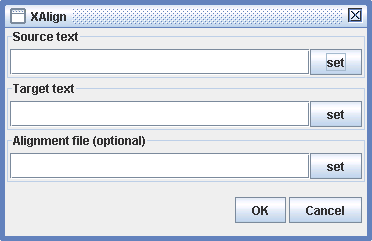
\includegraphics[width=9.5cm]{resources/img/figX-1.png}
\caption{Text alignment selection frame\label{fig-x-text-selection}}
\end{center}
\end{figure}

\begin{figure}[!ht]
\begin{center}
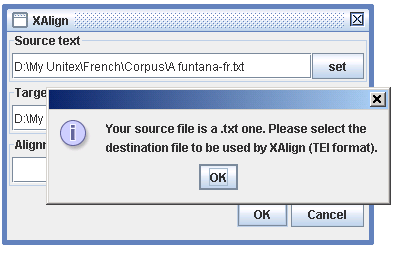
\includegraphics[width=10cm]{resources/img/figX-2.png}
\caption{Warning about raw texts\label{fig-x-tei-name}}
\end{center}
\end{figure}
\clearpage


\begin{figure}[!ht]
\begin{center}
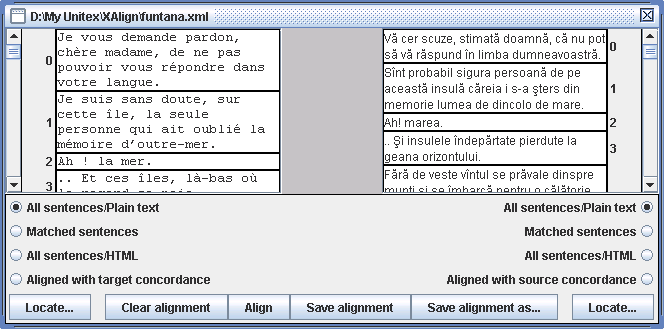
\includegraphics[width=15.5cm]{resources/img/figX-3.png}
\caption{Text alignment frame\label{fig-x-frame}}
\end{center}
\end{figure}

\section{Aligning texts}
Once you have loaded your texts, you can align them by clicking on the "Align"
button. You will be asked to provide the name of the XML file that will
contain all the information about the alignment. Then, Unitex launches the
\verb+XAlign+ program and you will visualize the alignment under the form of
red links between aligned sentences, as shown on Figure \ref{fig-x-links}.

\begin{figure}[!ht]
\begin{center}
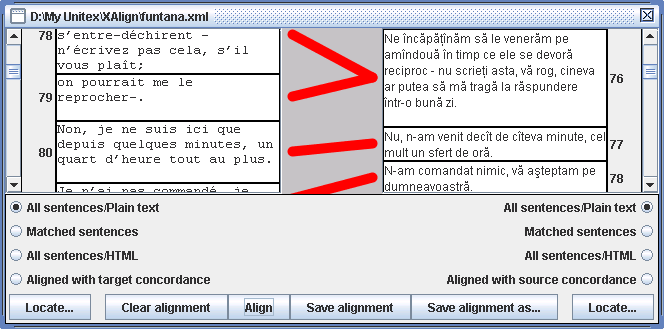
\includegraphics[width=15.5cm]{resources/img/figX-4.png}
\caption{Aligned sentences\label{fig-x-links}}
\end{center}
\end{figure}

\bigskip
\noindent You can edit the alignment links with the mouse. Clicking on a link
removes it. To add a link (or remove it, if it already exists), click on one
sentence (in the text you want, source or destination), and then move your mouse
over the corresponding sentence in the other text. The link about to be added
will appear in yellow, as shown on Figure \ref{fig-x-adding-a-link}. When you
click, the link is actually added and becomes red. When you have made all your
corrections, you can save your modified alignment using the "Save alignment"
and "Save alignment as\ldots" buttons.

\begin{figure}[!ht]
\begin{center}
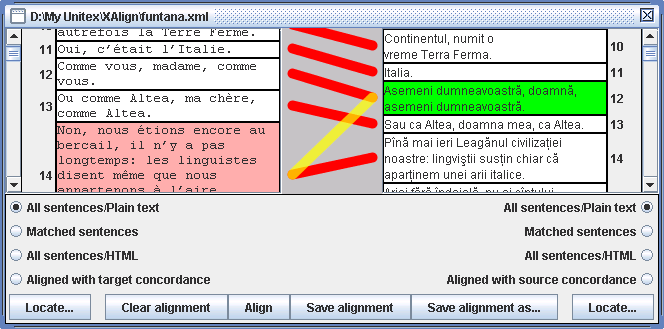
\includegraphics[width=15.5cm]{resources/img/figX-5.png}
\caption{Adding a link\label{fig-x-adding-a-link}}
\end{center}
\end{figure}

\bigskip
\noindent An interesting feature of XAlign is that it is
\textit{reentrant}.\index{Reentrant alignment} It means that you can take an
existing alignment as a set of mandatory links in input of the alignment
process. This can be useful if you want to work with
\textit{cognates}.\index{Cognates} For more details about cognates and XAlign,
see discussion in \cite{IGML_PauDum08}.

\clearpage
\section{Pattern matching}
You can perform pattern matching queries on any of your texts, by clicking on
its "Locate" button. The first time you click, Unitex will ask you to build a
working version of your text, as shown on Figure \ref{fig-x-fig6}. This text
version will be preprocessed according to the text language (in particular,
the default dictionaries will be applied).

\bigskip
\noindent WARNING: the text language is determined on the basis of the path
name. For instance, if your text file is located in \verb+.../MyUnitex/Klingon/Corpus+, 
the language will be considered to be \verb+Klingon+. So, if your text is not
in a subdirectory of your personal Unitex directory, its language will not be identified.

\begin{figure}[!ht]
\begin{center}
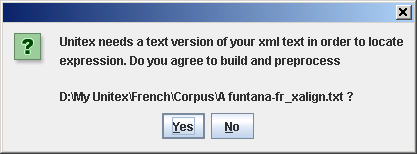
\includegraphics[width=10cm]{resources/img/figX-6.png}
\caption{Unitex needs to build a working version of your text\label{fig-x-fig6}}
\end{center}
\end{figure}
 
\begin{figure}[!ht]
\begin{center}
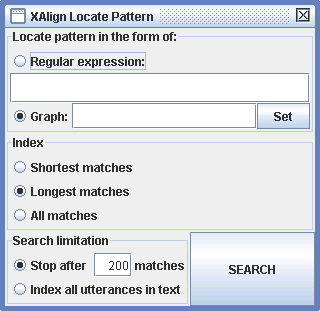
\includegraphics[width=7.8cm]{resources/img/figX-7.png}
\caption{Pattern matching frame for aligned texts\label{fig-x-locate-frame}}
\end{center}
\end{figure}

\bigskip
\noindent Once Unitex has created and preprocessed the working version of the
text, you can perform your query using the frame shown on Figure
\ref{fig-x-locate-frame}. As the matching operation is performed by the
\verb+Locate+ program,\index{\verb+Locate+} you can perform the same queries
than you would perform on a normal corpus. The only restriction is that you
cannot exploit the outputs of your grammars, if any.

\bigskip
\noindent For instance, let us lookup for the pattern \verb+<manger>+ 
(\textit {to eat}) in the French text of our example. First, we see no result,
because we have not changed yet the display mode for the French text, which 
by default is "All sentences/Plain text". Clicking on "Matched sentences", 
we only see sentences that contain occurrences, highlighted as usual in blue,
as shown on Figure \ref{fig-x-concord}. Clicking on "All sentences/HTML" will
display all sentences, highlighting occurrences in blue. 

\begin{figure}[!ht]
\begin{center}
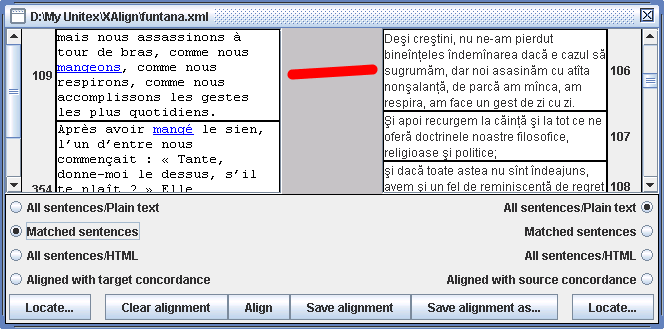
\includegraphics[width=15.5cm]{resources/img/figX-8.png}
\caption{Displaying matched sentences\label{fig-x-concord}}
\end{center}
\end{figure}

\bigskip
\noindent To exploit parallel texts, it is then interesting to retrieve
sentences aligned with matched sentences. This can be done by selecting
\textit{for the other text}, the display mode "Aligned with source
concordance". In this mode, Unitex filters sentences that are not linked
to matched sentences in the source text. So, it is easy to lookup for an
expression in one text and to find the corresponding sentences in the other,
as shown on Figure \ref{fig-x-concord-aligned}.

\begin{figure}[!ht]
\begin{center}
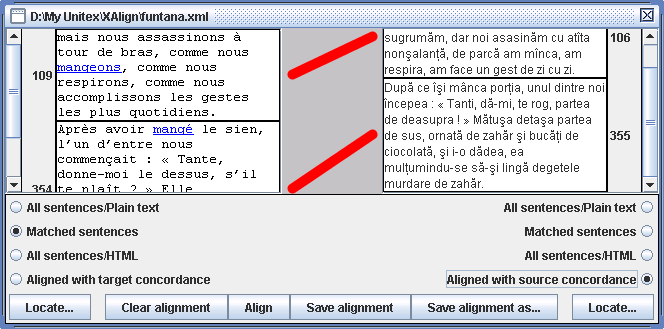
\includegraphics[width=15.5cm]{resources/img/figX-9.png}
\caption{Displaying matched sentences and sentences
they are linked to\label{fig-x-concord-aligned}}
\end{center}
\end{figure}
